% document formatting
\documentclass[10pt]{article}
\usepackage[utf8]{inputenc}
\usepackage[left=1in,right=1in,top=1in,bottom=1in]{geometry}
\usepackage[T1]{fontenc}
\usepackage{xcolor}

% math symbols, etc.
\usepackage{amsmath, amsfonts, amssymb, amsthm}

% lists
\usepackage{enumerate}

% images
\usepackage{graphicx} % for images

% code blocks
\usepackage{minted, listings} 

% verbatim greek
\usepackage{alphabeta}

\graphicspath{{./assets/images}}

\newcommand{\solution}{\textbf{Solution:}} 
\newcommand{\example}{\textbf{Example: }}

\title{EC ENGR 102 Week 4}

\author{Aidan Jan}
\date{\today}

\begin{document}
\maketitle

\subsection*{Using Commutativity to Show System Stability}
\begin{itemize}
    \item BIBO Stability: if $|x(t)| \leq M_x < \infty$ and $y(t) = H(x(t))$, then $H$ is BIBO stable if $|y(t)| \leq M_y < \infty$.
    \item Commutativity states:
    \begin{align*}
        |y(t)| &= \left|\int_{-\infty}^\infty x(\tau) h(t - \tau) \text{d}\tau\right|\\
        &= \left|\int_{-\infty}^\infty h(\tau) x(t - \tau) \text{d}\tau \right|
    \end{align*}

    [FILL]
\end{itemize}

\subsection*{Proof of Associativity}
Show that:
\[(f * (g * h))(t) = ((f * g) * h)(t)\]
First, note that
\[y(t - \alpha) = \int_{-\infty}^\infty x(\tau) h(t - \alpha - \tau) \text{d}\tau\]
as per the definition of the convolution.\\\\
Starting with the left-hand side:
\begin{align*}
f * (g * h)(t) &= \int_{-\infty}^\infty f(\tau_1) \cdot (g * h)(t - \tau_1) \text{d}\tau_1\\
&= \int_{-\infty}^\infty f(\tau_1) \cdot \int_{-\infty}^\infty g(\tau_2) h(t - \tau_1 - \tau_2) \text{ d}\tau_2 \text{ d}\tau_1\\
\intertext{Let $\tau_2 = \tau_3 - \tau_1$.  Therefore, $\tau_3 = \tau_1 + \tau_2$ and $\text{d}\tau_2 = \text{d}\tau_3$}\\
&= \int_{-\infty}^\infty f(\tau_1) \cdot \int_{-\infty}^\infty g(\tau_3 - \tau_1) \cdot h(t - \tau_3) \text{ d} \tau_3 \text{ d}\tau_1\\
\intertext{Now, we can change the order of integration.}\\
&= \int_{-\infty}^\infty h(t - \tau_3) \cdot \int_{-\infty}^\infty f(\tau_1) \cdot g(\tau_3 - \tau_1) \text{ d} \tau_1 \text{ d} \tau_3\\
&= \int_{-\infty}^\infty h(t - \tau_3) (f * g) (\tau_3) \text{ d}\tau_3\\
&= \int_{-\infty}^\infty (f * g)(\tau_3) h(t - \tau_3) \text{ d}\tau_3\\
&= (f * g) * h
\end{align*}

\subsection*{Proof of Distributivity}
Show that:
\[f * (g + h) = f * g + f * h\]
To prove this, we write out the definition of convolution:
\begin{align*}
    (f * (g + h))(t) &= \int_{-\infty}^\infty f(\tau)[g(t - \tau) + h(t - \tau)] \text{d}\tau\\
    &= \int_{-\infty}^\infty f(\tau) g(t - \tau) \text{d}\tau + \int_{-\infty}^\infty f(\tau) h(t - \tau) \text{d}\tau\\
    &= (f * g)(t) + (f * h)(t)
\end{align*}

\subsection*{Identity Element of Convolution}
Here, we have something that looks like an "algebra of signals," with addition like in ordinary algebra, and multiplication is replaced by convolution.  In standard algebra, the multiplicative identity is 1.  In signals, the convolution identity is the Dirac delta function, $\delta(t)$.\\\\
In particular, note that:
\[\boxed{x(t) * \delta(t) = x(t)}\]
because
\begin{align*}
    x(t) * \delta(t) &= \int_{-\infty}^\infty x(\tau) \delta(t - \tau) \text{d} \tau\\
    &= \int_{-\infty}^\infty \delta(\tau) x(t - \tau) \text{d}\tau\\
    &= \int_{-\infty}^\infty \delta(\tau)x(t) \text{d}\tau\\
    &= x(t)\int_{-\infty}^\infty \delta(\tau) \text{d}\tau\\
    &= x(t)
\end{align*}
\subsection*{Delay via Convolution}
Convolution with the impulse can also be used to delay signals, i.e.,
\[\boxed{x(t) * \delta(t - t_d) = x(t - t_d)}\]
To prove this, note that:
\[x(t) * \delta(t - t_d) = \int_{-\infty}^\infty x(\tau) \delta(t - t_d - \tau)\text{d}\tau\]
i.e., $x(\tau)$ is being multiplied by an impulse that occurs at $\tau = t - t_d$.  From what we know about convolution, this extracts out the value of $x(\tau)$ at $t - t_d$.\\
So,
\begin{align*}
    x(t) * \delta(t - t_d) &= \int_{-\infty}^\infty x(\tau) \delta(t - t_d - \tau) \text{d}\tau\\
    &= \int_{-\infty}^\infty x(t - t_d) \delta(t - t_d - \tau) \text{d}\tau\\
    &= x(t - t_d) \int_{-\infty}^\infty \delta(t - t_d - \tau) \text{d}\tau\\
    &= x(t - t_d)
\end{align*}

\subsection*{Integration Through Convolution}
Convolution can be used to implement integration.   In particular, to integrate a signla $x$ from $-\infty$ to $t$, we integrate it with a unit step.
\begin{align*}
    x(t) * u(t) &= \int_{-\infty}^\infty x(\tau) u(t - \tau) \text{d}\tau\\
    &= \int_{-\infty}^t x(\tau) \text{d}\tau
\end{align*}
where we used the fact that $u(t - \tau)$ is zero for when $\tau > t$.

\subsection*{Additional Properties of Convolution}
Given these properties of convolution, there are now a few properties we cah derive regarding convolution.
\begin{itemize}
    \item \textbf{Linearity:} Convolution is \textbf{linear}, since for all signals $x_1, x_2$ and all $\alpha, \beta \in \mathbb{R}$.
    \[h * (\alpha x_1 + \beta x_2) = \alpha(h * x_1) + \beta(h * x_2)\]
    \item \textbf{Time-invariance:} if $y(t) = x(t) * h(t)$, then if we delay the input by $T$, i.e., the new input is $x(t - T)$, then the output is $y(t - T)$.
    \item \textbf{Cascade (composition):} Due to the associativity of convolution, the cascade connection of two convolutions systems, $y = (x * f) * g$ is equivalent to a single system $y = x * h$, where $h = f * g$.  That is, the following two block diagrams are equivalent:
    \begin{center}
        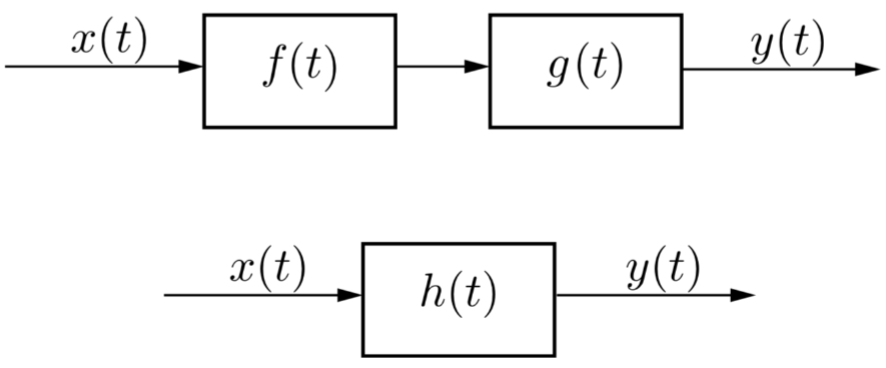
\includegraphics[scale=0.7]{W4_1.png}
    \end{center}
    \item \textbf{Swapping (composition II):} If $y = (x * f) * g$, then due to the commutivity of convolution, this is equivalent to $y = (x * g) * f$.  This means that you can swap the order of convolutions, as illustrated in the block diagram below:
    \begin{center}
        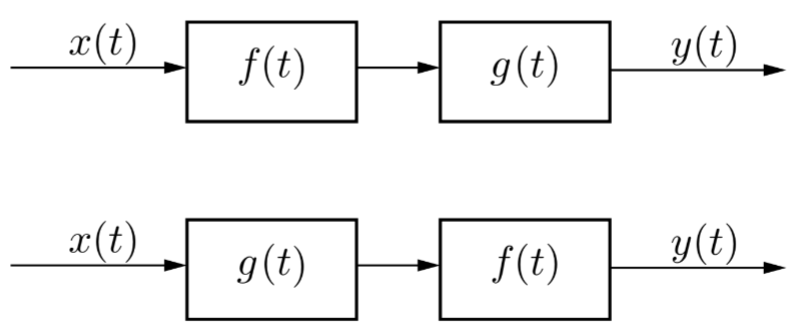
\includegraphics[scale=0.7]{W4_2.png}
    \end{center}
    Many operations can be written as convolutions (integration, delays, differentiation, etc.) and these operations all commute.
\end{itemize}

\subsubsection*{Question: How are the Impulse and Step Response related?}
\begin{center}
    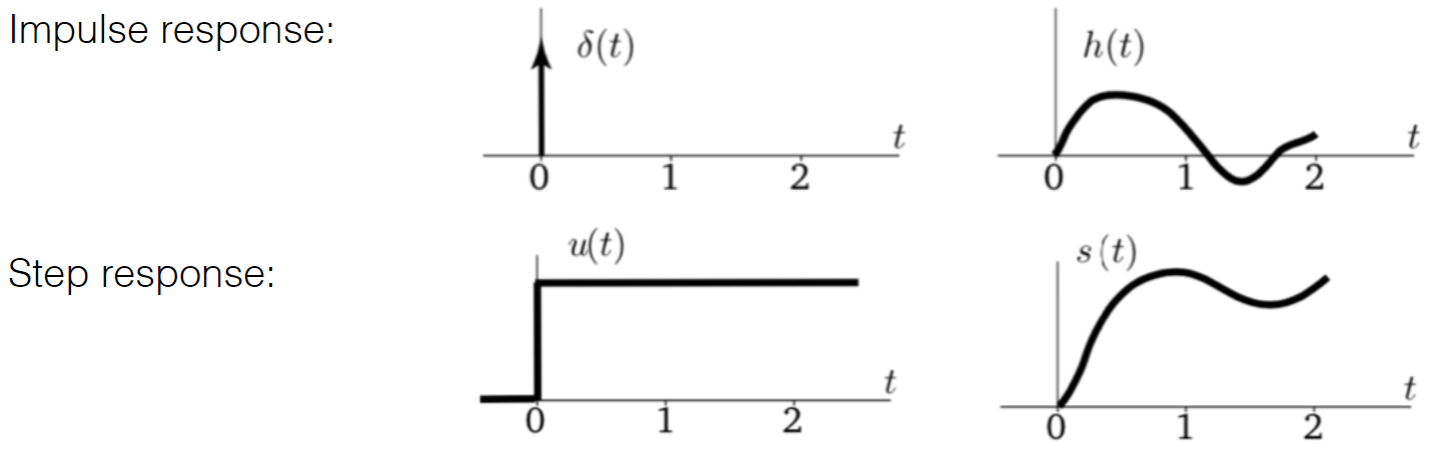
\includegraphics[scale=0.5]{W4_3.png}
\end{center}
It turns out that the integral of the impulse response is the step response!  (This makes sense since the integral of the Dirac delta function is the unit step.)\\
\hrulefill\\
Due to commutivity, we can now find the impulse response by differentiating the step response, i.e.,
\[h(t) = \frac{\text{d}s(t)}{\text{d}t}\]
This is illustrated below.
\begin{center}
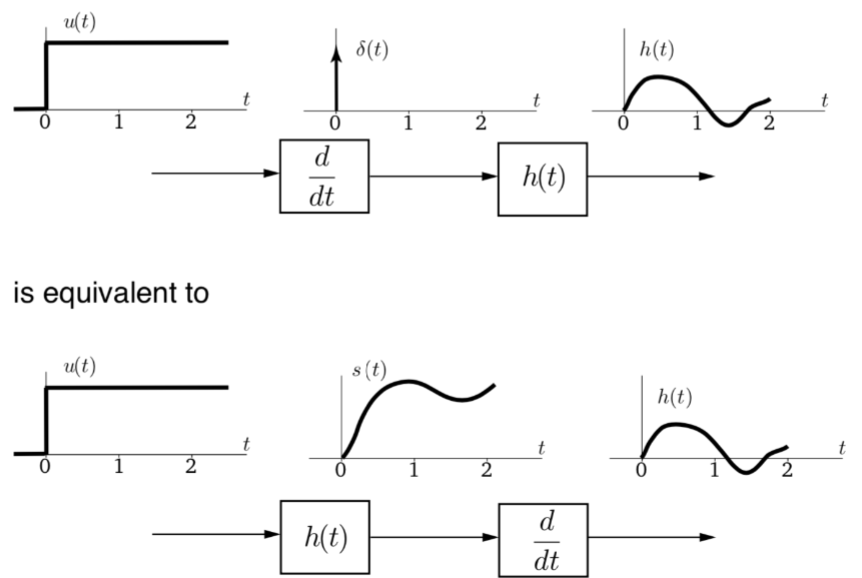
\includegraphics[scale=0.5]{W4_4.png}
\end{center}

\subsection*{Recap on LTI Systems and Convolution}
\begin{enumerate}
    \item \textbf{Any LTI system can be characterized by an impulse response.}\\\\
    This means that if I know the impulse response, I can calculate the output of the system for any given input.\\\\
    \textit{Example application:} consider playing baseball.  Swinging the bat, and making contact with a ball is like a brief impulse (force) applied from the bat to the ball.  How the ball flies through the air is an example of an impulse response.\\\\
    \textit{Example application:} consider a stringed instrument.  When I pluck the string, it begins to vibrate.  Its vibration is an impulse response.\\\\
    \textbf{Step responses} are more common.\\\\
    \textit{Example application:} I step on the gas pedal of my car.  The car's response is an example of a step response, and it looks different depending on the car (e.g., an EV vs. a gas car).\\\\
    \textit{Example application:} I flip a switch, which turns on the power to a circuit.  How the circuit acts when I flip the switch is its step response.
    \item To calculate the impulse response, we input an impulse to the system and measure the output.
    \item After we know the impulse response, we can caltulate the output for any given input via the convolution integral.
    \[\boxed{y(t) = \int_{-\infty}^\infty x(\tau) h(t - \tau) \text{d}\tau}\]
    \item This operation has several properties.
    \begin{itemize}
        \item Commutativity
        \item Associativity
        \item Distributivity
        \item Identity Element
        \item Delay
        \item LTI
        \item Composition
    \end{itemize}
\end{enumerate}

\subsubsection*{Other Examples of Swapping:}
\begin{itemize}
    \item Say I wanted to edit a piece of music by making the treble quieter.  After this, I still wasn't happy with the recording and wanted to make the bass louder.  These happen to both be LTI operations and can be done in either order.
    \item Say I have an LTI circuit, and I want to know what happens when it receives a jolt of brief power (e.g., from a temporary power surge).  I can estimate this by giving it constant power input (a step), and then differentiating the circuit's response to the step.
\end{itemize}

\section*{Fourier Series}
\begin{itemize}
    \item Any periodic signal can be expressed as a sum of sinusoids. (complex exponentials).
    \item The sinusoids that make up the signal are called the Fourier Series.
    \item In terms of math,
    \[x(t) = x_1(t) + x_2(t) + \dots\]
    where each $x_i(t)$ is written in the form $e^{j\omega t} = \cos(\omega t) + j \cdot \sin(\omega t)$
\end{itemize}

\subsection*{Bottom Line}
If $f(t)$ is a well-behaved (continuous) periodic signal with period $T_0$, then $f(t)$ can be written as a Fourier series
\[\boxed{f(t) = \sum_{k = -\infty}^\infty c_k e^{jk\omega_0 t}}\]
where $\omega_0 = \frac{2\pi}{T_0}$ and
\[\boxed{c_k = \frac{1}{T_0} \int_\tau^{\tau + T_0} f(t) e^{-jk\omega_o t}\text{d}t}\]
for all integers $k$.  The $c_k$ are called the \textit{Fourier coefficients} of $f(t)$.\\\\
Here, $f(t)$ is the \textit{weighted average} of complex exponentials (which are simply complex sines and cosines).

\subsection*{Implications for LTI Systems}
We know that for a linear system, if $x(t) = x_1(t) + x_2(t) + \cdots + x_n(t)$, then
\begin{align*}
    y(t) &= h(t) * x(t)\\
    &= h(t) * (x_1(t) + x_2(t) + \cdots + x_n(t))\\
    &= h(t) * x_1(t) + h(t) * x_2(t) + \dots h(t) * x_n(t)
\end{align*}
What this tells us is that if we can decompose our signal, $x(t)$, into its components, we can calculate the system output by considering each of these components in isolation.  After this, we sum the outputs of these components together.\\\\
Fourier's idea, in 1807, was to decompose $x(t)$ using one of the most basic signals we know of: sines and cosines.

\subsection*{Eigenfunctions of LTI systems}
\begin{itemize}
    \item $x(t)$ is an \textit{eigenfunction} of a system, if, when inputting $x(t)$ to the system, the output is simply a scaled version of $x(t)$, i.e., $y(t) = ax(t)$ where $a$ is a constant (called an eigenvalue).  Note that $a$ may be a complex constant.
    \item \textbf{Complex exponentials are eigenfunctions of LTI systems}
    \begin{itemize}
        \item When a complex exponential (eigenfunction) is input into an LTI function, the resulting function is \textbf{always} the same function, possibly with amplitude and phase angle changes.  The frequency remains the same.
    \end{itemize}
\end{itemize}

\pagebreak
\subsection*{Deriving the Eigenfunctions of LTI Systems}
Consider an LTI system with impulse response $h(t)$.  If the input is a complex exponential, i.e., $e^{st}$ where $s = \sigma + j\omega$, then
\[y(t) = \int_{-\infty}^\infty h(\tau) e^{s(t - \tau)}\text{d}\tau\]
We can start by splitting up the exponent.

\begin{align*}
    y(t) &= \int_{-\infty}^\infty h(t) e^{st} \cdot e^{-s\tau} \text{d}\tau\\
    &= e^{st} \cdot \int_{-\infty}^\infty h(\tau) e^{-s\tau} \text{d}\tau\\
    \intertext{Notice that the integral is now a function of $s$.  There are no other variables present in there (also not dependent on $t$).  Therefore, we can write it as such.}
    &= H(s) \cdot e^{st}
\end{align*}
where $H(s) = \int_{-\infty}^\infty h(\tau) e^{-s\tau} \text{d}\tau$, called the "Transfer Function".


\end{document}